\chapter{Implementation}
\label{chap:implementation}

This section describes the artefact development process. Despite multiple stumbling blocks during development, these were overcome through problem-solving, thorough investigation and reading of software documentation.  

\section{Development Environment}
\label{implementation:de}

Visual Studio Code (VS Code) was chosen as the development environment for development (\cite{noauthor_visual_nodate}). VS Code was chosen due to its flexibility in working with multiple programming languages through the use of extensions. The React.js Framework, JavaScript and Go Language extensions were installed to ensure seamless development of the backend and frontend of the artefact. The ESLint extension was also used using Go and JavaScript configurations to ensure the consistency and readability of the codebase.

\section{Iteration 1 - Basic UI and Core Routing}
\label{implementation:iteration1}
The initial stages of development began using a first draft of elicited requirements \see{appendix:initial-user-requirements} where later in the project, a new set of user requirements was formed based on primary research. This method proved effective in not delaying initial development, where the core requirements were unlikely to change greatly. Furthermore, Iteration 1 consisted of implementing the building blocks of the artefact, including setting up a React.js App, Gin Webserver, PostgreSQL database and the core routing functionalities.

\subsection{Leaflet - Open Street Map (OSM)}
\label{iteration1:leaflet-osm}
The Map component was the first to be developed because the rest of the artefact would be dependent on its mapping functionality. The component contained a div element containing the MapContainer component imported from React Leaflet (\cite{noauthor_react_nodate}). The component includes a tile layer to make API requests to Open Street Map (\cite{noauthor_openstreetmap_nodate}) to get the tile images for the map, and then display these tiles to form the full-screen map element. Temporary variables were set up to store the latitude and longitude values representing the start and end of a route, then drawn on the map using a polyline and marker points \see{fig:basic-map-with-route}. 

\begin{figure}[!ht]
    \centering
    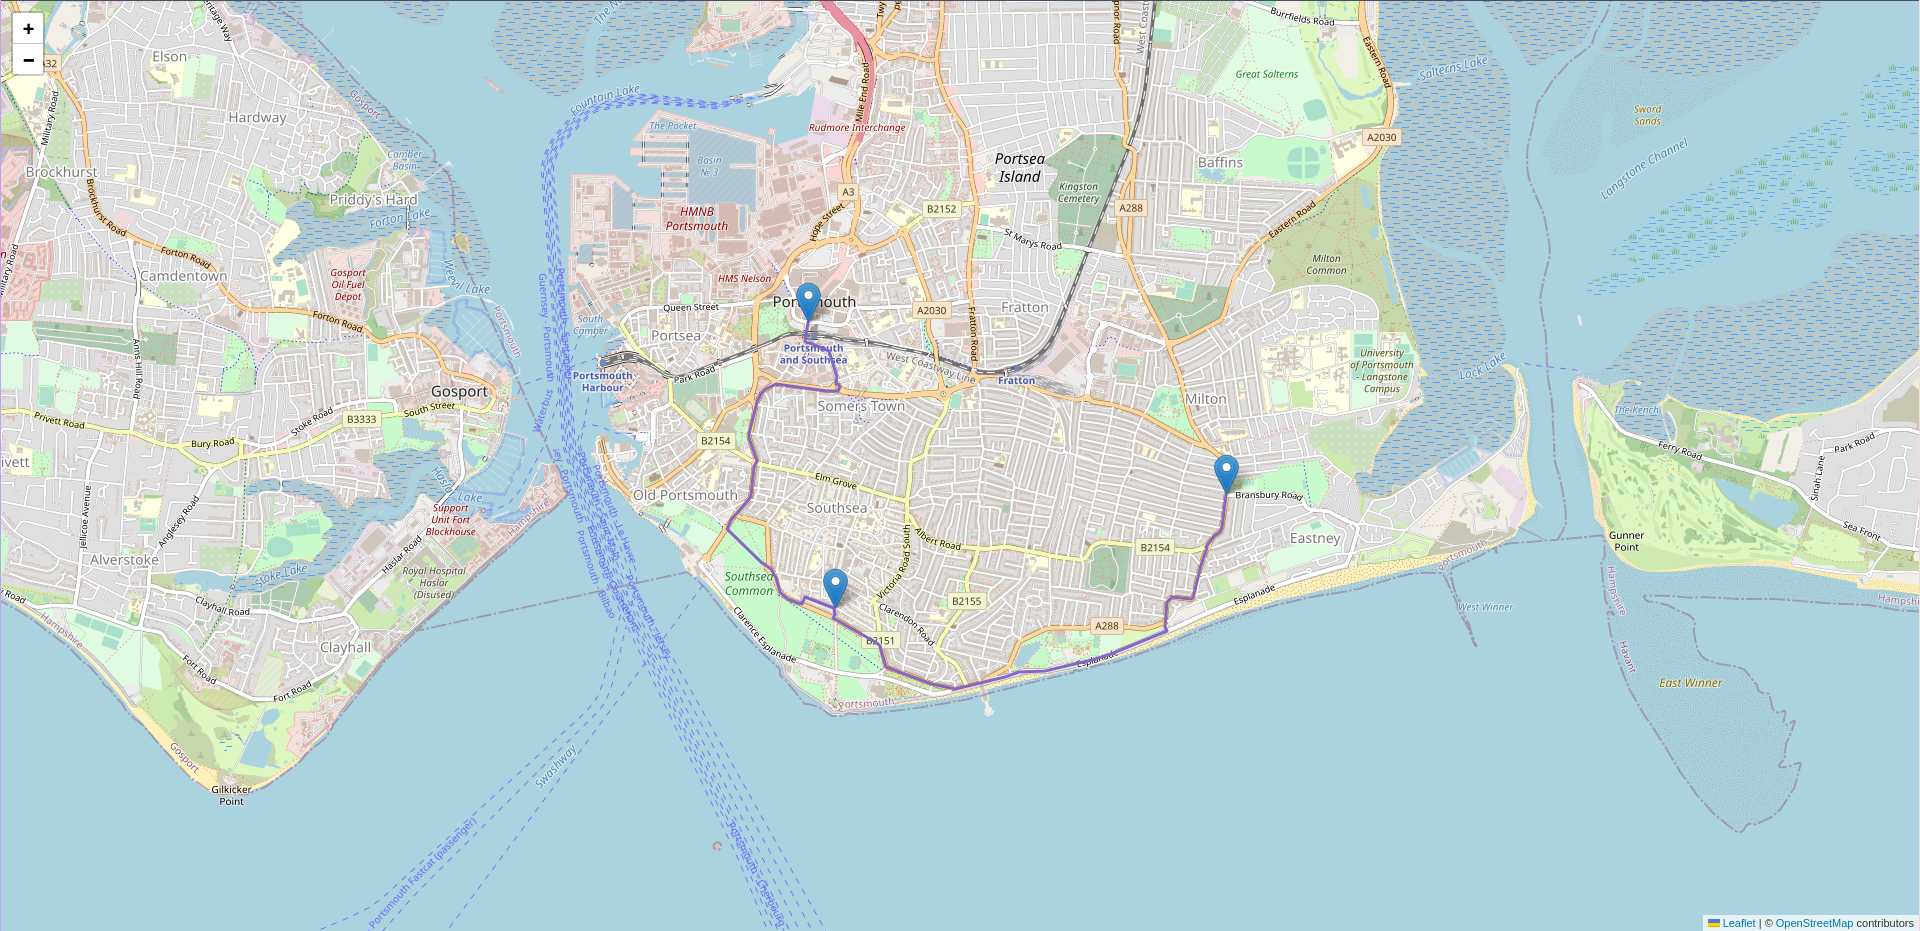
\includegraphics[width=425px]{figures/Progress Images/Iteration-1/SR25/Basic Route.png}
    \caption{Basic Map with Route}
    \label{fig:basic-map-with-route}
\end{figure}

\subsection{Basic Route Planning}
\label{iteration1:basic-routing}
After conducting research, the most effective way to implement route planning with Leaflet was to use Leaflet Routing Machine (\cite{noauthor_leaflet_nodate-1}). This library enabled a RoutingMachine component to be natively added on top of the React Leaflet map component, whilst providing a basic, customisable route planning UI \see{fig:routing-ui}. The routing API in use at the beginning was Open Source Routing Machine (OSRM) (\cite{noauthor_project_nodate}) which appeared to meet all requirements of a routing algorithm until round trip routing was required \see{implementation:iteration2}. This new routing functionality enabled the user to select a start, destination and any intermediate locations, a route would then be planned. At this stage, the route could be altered through the use of waypoints, but the artefact did not provide any further custom routing features to the user.
\begin{figure}[!ht]
    \centering
    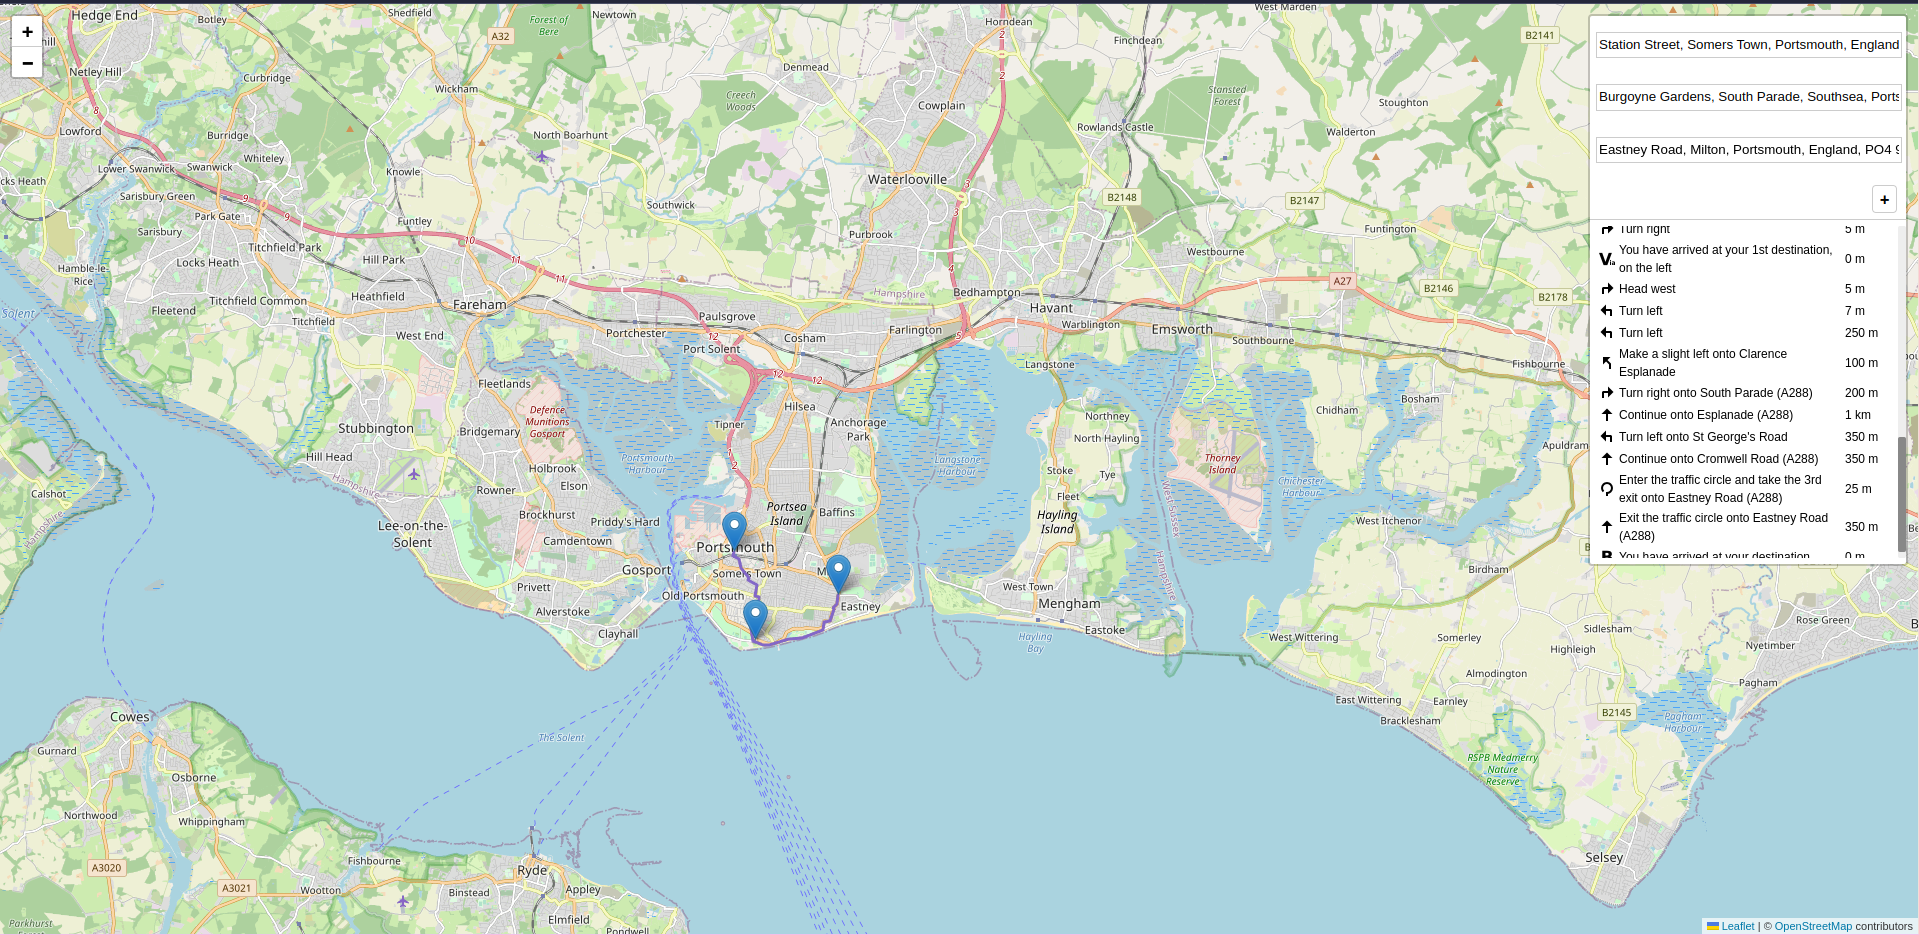
\includegraphics[width=425px]{figures/Progress Images/Iteration-1/SR1/Basic Destination Overlay Set up.png}
    \caption{Routing UI}
    \label{fig:routing-ui}
  \end{figure}

\subsection{Elevation Chart}
\label{iteration1:elevation-chart}
To create an elevation chart, the component was declared, with the plan to use Chart.js (\cite{noauthor_chartjs_nodate}) to draw the plot on a canvas element. A div was created to hold the chart component, where the elevation data was gathered from a state variable called 'coordinates' which contained the route latitude, longitude points and the altitude/elevations for each point \see{fig:waypoint-arr}. The distance along the route for each elevation point is calculated by dividing the total route distance (taken from a state variable called 'summary') by the length of the 'coordinates' array. To ensure continuity between the map and the elevation plot, a simple feature was added to allow the user to hover over the elevation plot, with the matching point along the route being highlighted. This required the hover point on the chart's canvas element to be found, matching the hover value to the latitude and longitude with the respective point and drawing a circle element on the Leaflet map \see{fig:elevation-hover}.

\begin{figure}[!ht]
    \centering
    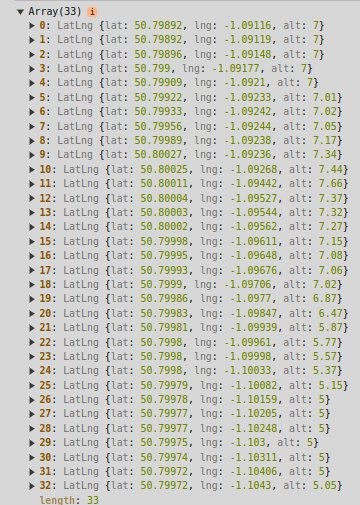
\includegraphics[width=200px]{figures/Progress Images/Iteration-1/SR1/waypoint-arr.png}
    \caption{Route Waypoint/Elevation Array}
    \label{fig:waypoint-arr}
  \end{figure}

\begin{figure}[!ht]
    \centering
    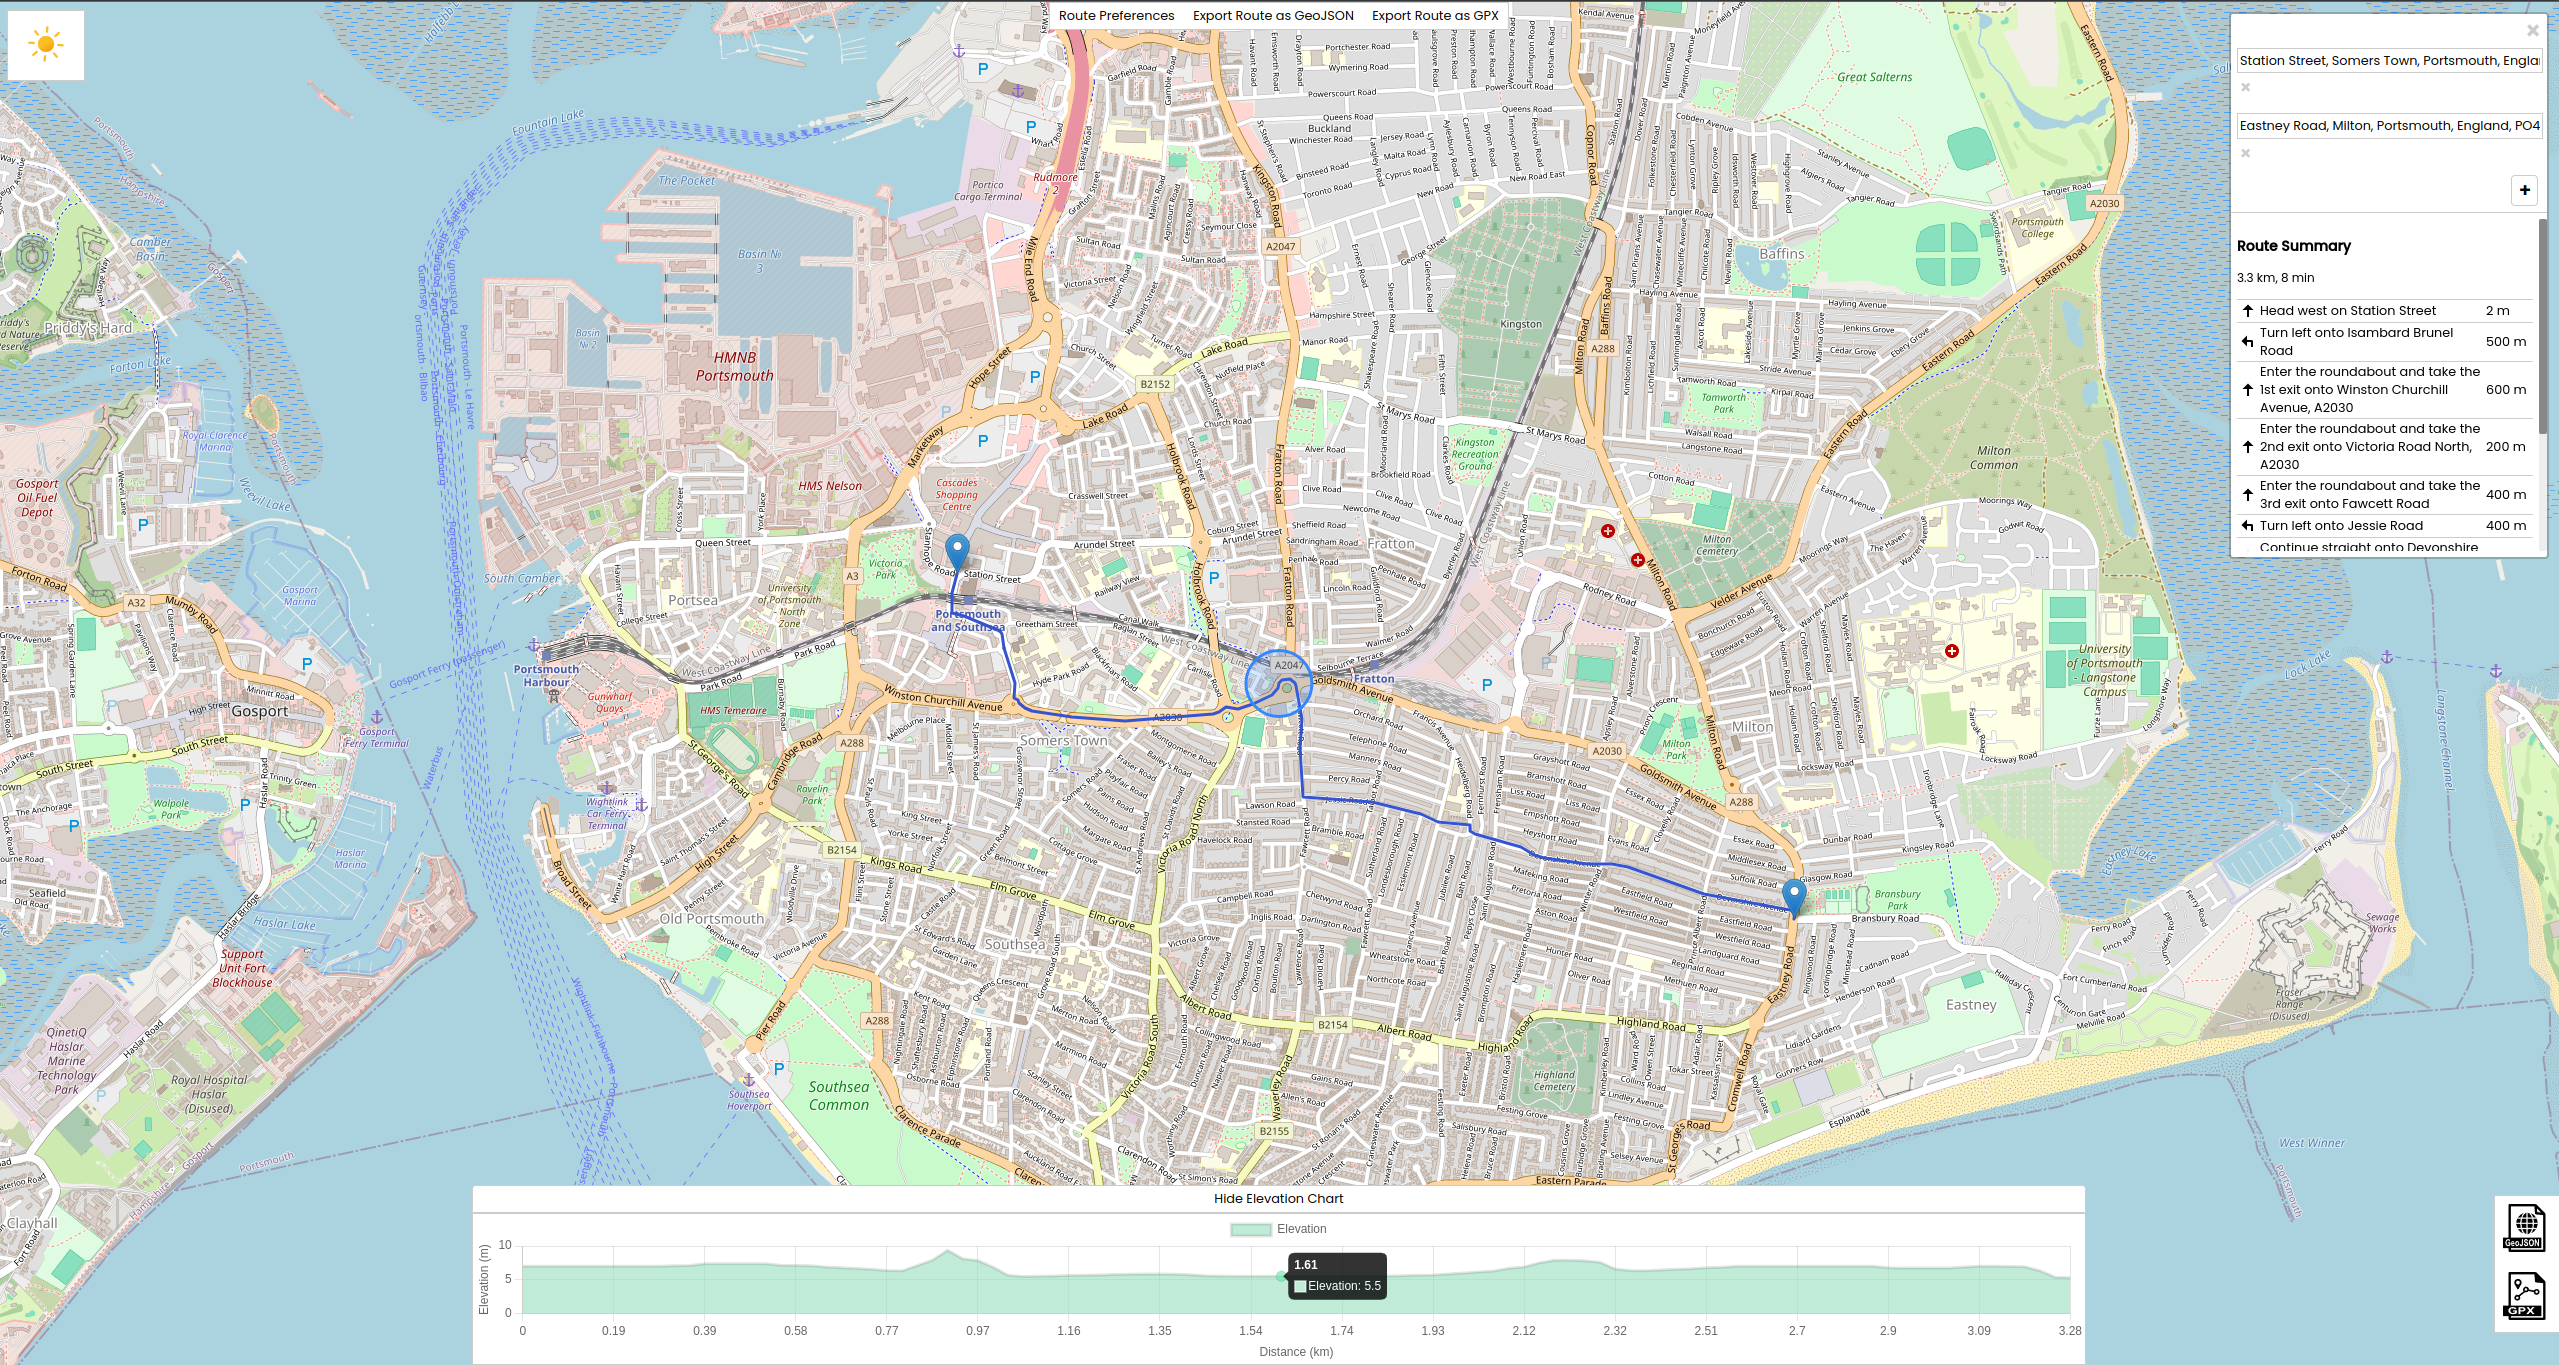
\includegraphics[width=425px]{figures/Progress Images/Iteration-1/SR28/elevation-hover.png}
    \caption{Elevation Plot Hover Functionality}
    \label{fig:elevation-hover}
\end{figure}

\subsection{Weather Information Panel}
\label{iteration1:weather-panel}
A generic weather panel was created within iteration 1, displaying weather information for the current day at the user's current location. The weather panel used the browser's geolocation API called within a React useEffect to get the user's general location, asking for permission via a pop-up window, then storing the geolocation in a state variable. The approximate coordinates returned from the API were then passed to Open Weather Map to gather all weather data for the current day. The Meteocons icons (\cite{noauthor_weather_nodate}) were used to display images demonstrating the current weather conditions \see{fig:basic-weather-panel}. The visibility of the weather panel was determined by a State variable, if the variable was true, the height and width of the panel expand, and when false, reduce to the button size.

\begin{figure}[!ht]
    \centering
    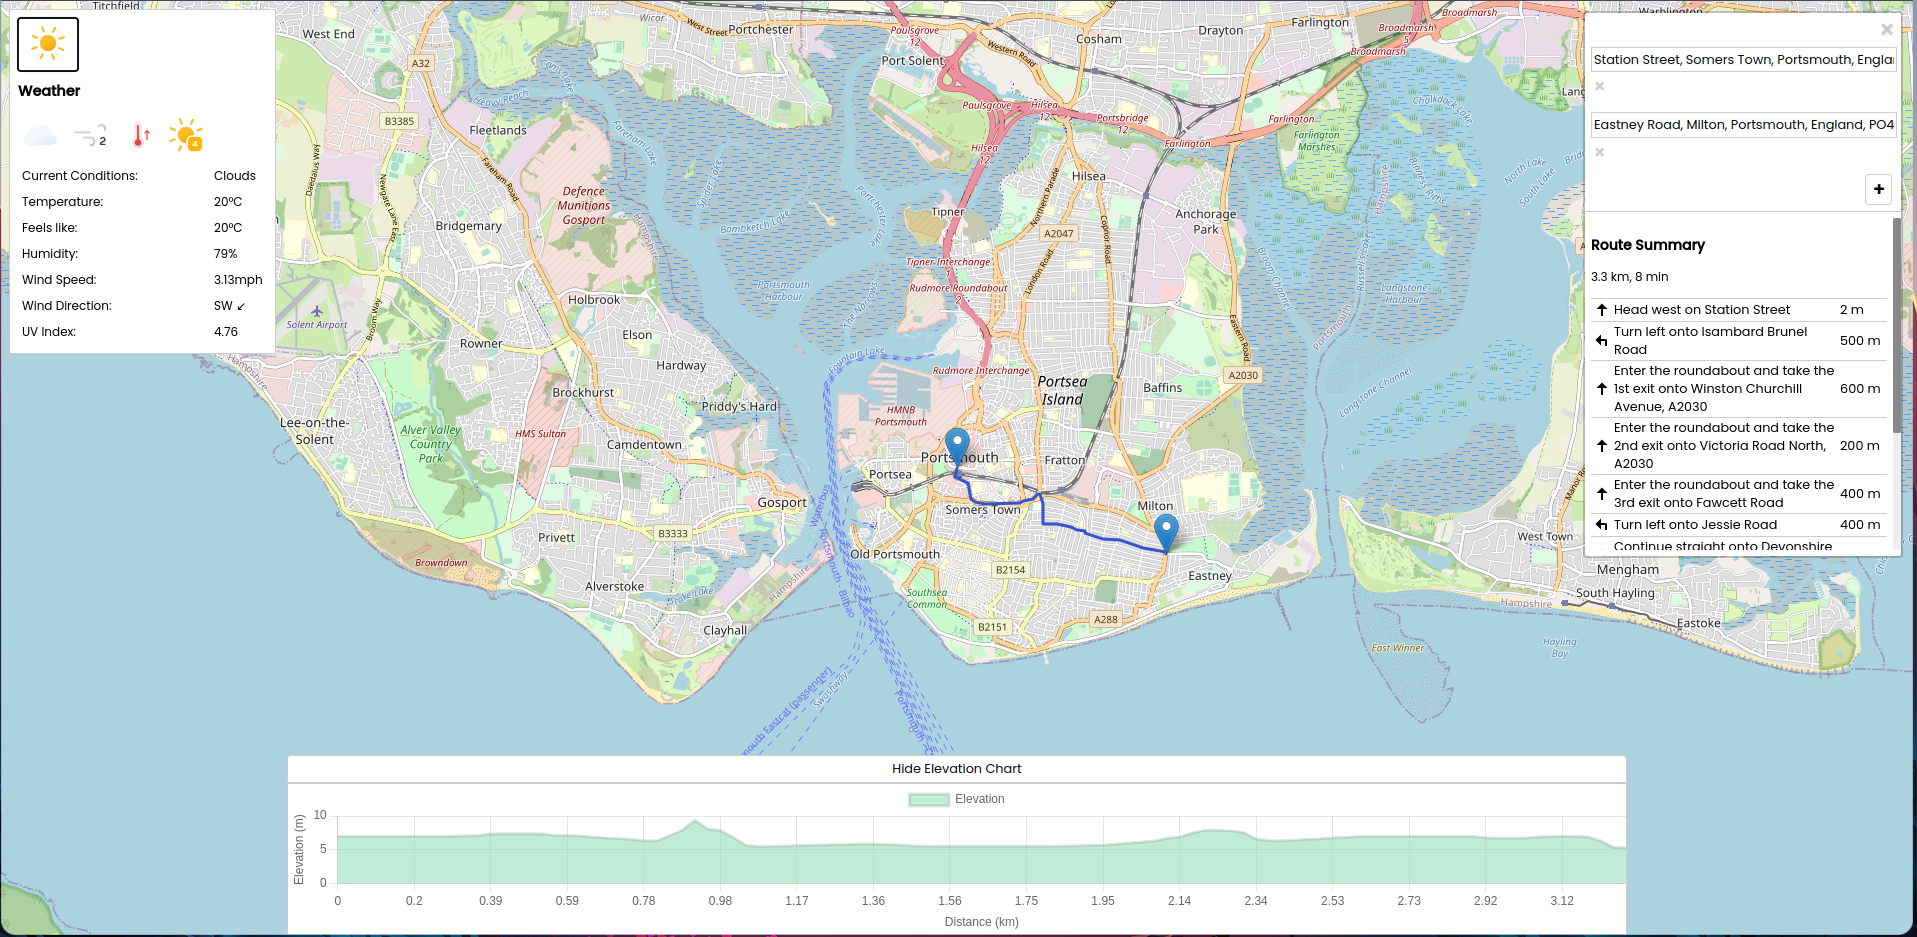
\includegraphics[width=425px]{figures/Progress Images/Iteration-1/SR19&SR28 Combined/SR19&SR28 Merged.png}
    \caption{Weather Panel}
    \label{fig:basic-weather-panel}
\end{figure}

\subsection{Main Challenges}
\label{iteration1:main-challenges}
The main challenge of Iteration 1 (i1), was primarily integrating multiple services to communicate seamlessly through the React.js frontend. Syncing hovering over the elevation plot, with a matching point along the route polyline, proved difficult. Despite the calculations being simple to determine at what latitude and longitude to draw the circle marker on the map when hovering on the plot, getting the map instance reference was more difficult than expected. Initially, the reference would return undefined, therefore no marker was drawn on the map, however after implementing a useState and declaring a local copy of the map instance, the hover functionality worked seamlessly.

Furthermore, the only other challenge faced was retrieving the user's geolocation from the browser. A useEffect was required to access the geolocation API, however, the useState was at first missed to store the geolocation value once the API had returned the data. Once the state variable was added, however, the weather panel would re-render once the data was retrieved.

\section{Iteration 2}
\label{implementation:iteration2}

Unlike i1, the development of Iteration 2 (i2) was conducted after the primary research and requirements review had been completed. The remaining updated requirements were organised in order of priority and distributed between i2 and Iteration 3 (i3) \see{implementation:iteration3}. I2 builds on i1, enhancing existing functionality and introducing new features throughout the iteration.

\section{Iteration 3}
\label{implementation:iteration3}
